%!TEX root = ../dokumentation.tex

\section{Klassendiagramm}

\begin{figure}[!htbp]
	\centering
	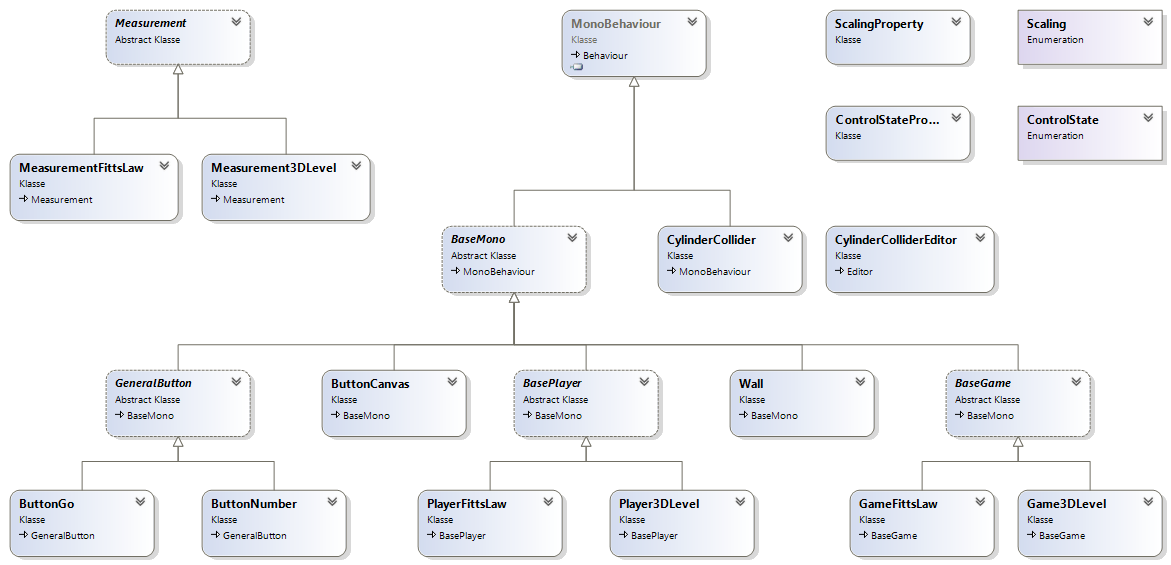
\includegraphics[angle=90,height=0.9\textheight]{ClassDiagram}
	\caption[Übersicht Klassenhierarchie]{Übersicht Klassenhierarchie}
	\label{fig:ClassDiagram}
\end{figure}

\section{Tabelle der Versuche}
% Please add the following required packages to your document preamble:
% \usepackage{booktabs}
% \usepackage{graphicx}

\begin{table}[H]	
	\caption{Tabelle der Versuche}
	\label{table:probanden}
	\resizebox{\textwidth}{!}{%
		\begin{tabular}{@{}lllll@{}}
			\toprule
			Proband & Laserpointer und Trigger & Laserpointer und Blinzeln & Eye-Tracking und Trigger & Eye-Tracking und Blinzeln \\ \midrule
			1  & (3, 2), (2, 2), (3, 3) & (3, 2), (1, 2), (3, 3) & (3, 4), (2, 4), (3, 2) & (2, 3), (1, 3), (2, 1) \\
			2  & (1, 3), (3, 3), (1, 4) & (2, 1), (1, 1), (2, 3) & (1, 3), (2, 3), (1, 2) & (3, 2), (1, 2), (3, 4) \\
			3  & (1, 4), (2, 4), (1, 3) & (1, 4), (3, 4), (1, 3) & (1, 1), (2, 1), (1, 3) & (1, 4), (2, 4), (1, 3) \\
			4  & (3, 4), (1, 4), (3, 1) & (2, 4), (3, 4), (2, 1) & (2, 3), (3, 3), (2, 2) & (1, 1), (3, 1), (1, 2) \\
			5  & (3, 1), (1, 1), (3, 3) & (2, 3), (3, 3), (2, 4) & (1, 3), (3, 3), (1, 2) & (3, 1), (1, 1), (3, 2) \\
			6  & (2, 2), (3, 2), (2, 3) & (3, 1), (2, 1), (3, 4) & (3, 2), (1, 2), (3, 1) & (2, 2), (3, 2), (2, 3) \\
			7  & (2, 1), (3, 1), (2, 4) & (2, 2), (3, 2), (2, 4) & (2, 4), (3, 4), (2, 2) & (3, 3), (2, 3), (3, 2) \\
			8  & (2, 4), (3, 4), (2, 3) & (2, 1), (3, 1), (2, 4) & (2, 3), (3, 3), (2, 4) & (3, 4), (1, 4), (3, 3) \\
			9  & (1, 1), (2, 1), (1, 4) & (1, 2), (2, 2), (1, 4) & (2, 1), (1, 1), (2, 2) & (1, 2), (2, 2), (1, 1) \\
			10 & (3, 1), (2, 1), (3, 3) & (1, 2), (3, 2), (1, 3) & (3, 1), (2, 1), (3, 3) & (2, 1), (1, 1), (2, 2) \\
			11 & (2, 1), (3, 1), (2, 4) & (3, 1), (1, 1), (3, 3) & (1, 4), (2, 4), (1, 2) & (2, 2), (3, 2), (2, 4) \\
			12 & (1, 4), (3, 4), (1, 1) & (1, 1), (3, 1), (1, 4) & (3, 4), (1, 4), (3, 1) & (2, 4), (3, 4), (2, 3) \\
			13 & (1, 2), (2, 2), (1, 1) & (2, 2), (1, 2), (2, 3) & (3, 1), (1, 1), (3, 2) & (1, 4), (3, 4), (1, 2) \\
			14 & (3, 2), (2, 2), (3, 4) & (2, 2), (3, 2), (2, 3) & (3, 4), (1, 4), (3, 2) & (3, 3), (1, 3), (3, 1) \\
			15 & (3, 3), (2, 3), (3, 2) & (1, 4), (3, 4), (1, 3) & (2, 1), (1, 1), (2, 2) & (2, 1), (3, 1), (2, 4) \\
			16 & (1, 3), (2, 3), (1, 2) & (1, 3), (3, 3), (1, 4) & (3, 4), (1, 4), (3, 1) & (2, 1), (3, 1), (2, 2) \\
			17 & (1, 2), (2, 2), (1, 1) & (2, 1), (1, 1), (2, 4) & (2, 2), (1, 2), (2, 3) & (1, 4), (2, 4), (1, 1) \\
			18 & (2, 4), (3, 4), (2, 1) & (3, 3), (1, 3), (3, 4) & (1, 3), (2, 3), (1, 1) & (1, 4), (3, 4), (1, 3) \\
			19 & (1, 2), (3, 2), (1, 3) & (2, 2), (1, 2), (2, 3) & (2, 4), (1, 4), (2, 1) & (1, 3), (3, 3), (1, 2) \\
			20 & (1, 3), (2, 3), (1, 2) & (3, 1), (1, 1), (3, 2) & (3, 3), (1, 3), (3, 2) & (2, 3), (3, 3), (2, 1) \\ \bottomrule
		\end{tabular}%
	}
\end{table}

\section{Tabellen der Befragungsergebnisse}
\label{appendix:tables}

\begin{table}[]
	\caption{Angaben der Probanden zu Laserpointer/Trigger}
	\resizebox{\textwidth}{!}{%
		\begin{tabular}{|l|l|l|l|l|}
			\hline
			\multirow{2}{*}{Proband} & \multicolumn{4}{l|}{Laserpointer/Trigger}                         \\ \cline{2-5} 
			& Fixierung & Auswahl & Eignung Menüsteuerung & Einfluss Knopfgröße \\ \hline
			Proband 1                & 5         & 5       & 5                     & 2                   \\ \hline
			Proband 2                & 5         & 5       & 5                     & 2                   \\ \hline
			Proband 3                & 5         & 5       & 5                     & 2                   \\ \hline
			Proband 4                & 5         & 5       & 5                     & 2                   \\ \hline
		\end{tabular}%
	}
\end{table}

\begin{table}[]
	\caption{Angaben der Probanden zu Laserpointer/Blinzeln}
	\resizebox{\textwidth}{!}{%
		\begin{tabular}{|l|l|l|l|l|}
			\hline
			\multirow{2}{*}{Proband} & \multicolumn{4}{l|}{Laserpointer/Blinzeln}                        \\ \cline{2-5} 
			& Fixierung & Auswahl & Eignung Menüsteuerung & Einfluss Knopfgröße \\ \hline
			Proband 1                & 5         & 3       & 4                     & 3                   \\ \hline
			Proband 2                & 5         & 4       & 5                     & 2                   \\ \hline
			Proband 3                & 5         & 5       & 4                     & 2                   \\ \hline
			Proband 4                & 5         & 1       & 1                     & 2                   \\ \hline
		\end{tabular}%
	}
\end{table}

\begin{table}[]
	\caption{Angaben der Probanden zu Eye-Tracking/Trigger}
	\resizebox{\textwidth}{!}{%
		\begin{tabular}{|l|l|l|l|l|}
			\hline
			\multirow{2}{*}{Proband} & \multicolumn{4}{l|}{Eye-Tracking/Trigger}                         \\ \cline{2-5} 
			& Fixierung & Auswahl & Eignung Menüsteuerung & Einfluss Knopfgröße \\ \hline
			Proband 1                & 3         & 4       & 4                     & 4                   \\ \hline
			Proband 2                & 4         & 4       & 5                     & 3                   \\ \hline
			Proband 3                & 2         & 4       & 3                     & 4                   \\ \hline
			Proband 4                & 4         & 4       & 5                     & 4                   \\ \hline
		\end{tabular}%
	}
\end{table}

\begin{table}[]
	\caption{Angaben der Probanden zu Eye-Tracking/Blinzeln}
	\resizebox{\textwidth}{!}{%
		\begin{tabular}{|l|l|l|l|l|}
			\hline
			\multirow{2}{*}{Proband} & \multicolumn{4}{l|}{Eye-Tracking/Blinzeln}                         \\ \cline{2-5} 
			& Fixierung & Auswahl & Eignung Menüsteuerung & Einfluss Knopfgröße \\ \hline
			Proband 1                & 1         & 1       & 1                     & 5                   \\ \hline
			Proband 2                & 1         & 1       & 1                     & 5                   \\ \hline
			Proband 3                & 2         & 1       & 1                     & 5                   \\ \hline
			Proband 4                & 1         & 1       & 1                     & 5                   \\ \hline
		\end{tabular}%
	}
\end{table}

\begin{table}[]
	\resizebox{\textwidth}{!}{%
		\begin{tabular}{|l|l|l|l|l|}
			\hline
			\multirow{2}{*}{Proband} &
			\multicolumn{4}{l|}{Ranking und Begründung} \\ \cline{2-5} 
			&
			Ranking &
			Begründung 1. Platz &
			Begründung 2. Platz &
			Begründung 4. Platz \\ \hline
			Proband 1 &
			1, 2, 3, 4 &
			\begin{tabular}[c]{@{}l@{}}Fühlt sich intuitiv an, ist \\ am einfachsten zu bedienen \\ und funktioniert auf Anhieb.\end{tabular} &
			\begin{tabular}[c]{@{}l@{}}das Blinzeln als Alternative \\ zum Trigger hat \\ auch sehr gut funktioniert.\end{tabular} &
			\begin{tabular}[c]{@{}l@{}}Eye-Tracking mit Blinzeln \\ hat überhaupt nicht funktioniert \\ und war eines der qualvollsten \\ Erlebnisse meines Lebens.\end{tabular} \\ \hline
			Proband 2 &
			1, 2, 3, 4 &
			\begin{tabular}[c]{@{}l@{}}Für mich als geübten \\ VR-Nutzer mit Abstand \\ am intuitivsten\end{tabular} &
			\begin{tabular}[c]{@{}l@{}}Die Genauigkeit der \\ Laserpointers mit der einfachen \\ Interaktion durch blinzeln hat \\ sehr gut funktioniert\end{tabular} &
			\begin{tabular}[c]{@{}l@{}}Fixierung war sehr schwer, \\ ich habe oft nicht den Knopf \\ getroffen, den ich treffen wollte. \\ Beim Blinzeln ist die Position \\ des Eye-Trackers oft verrutscht, \\ so dass ein genaues Treffen der \\ Knöpfe praktisch unmöglich war\end{tabular} \\ \hline
			Proband 3 &
			1, 2, 3, 4 &
			\begin{tabular}[c]{@{}l@{}}Beim Laserpointer wusste \\ man immer genau wohin \\ man zielte. Das Bestätigen \\ mit dem Trigger funktionierte \\ immer direkt auf Anhieb.\end{tabular} &
			\begin{tabular}[c]{@{}l@{}}Der Unterschied zu Nummer 1 \\ ist, dass das Blinzeln nicht \\ immer direkt auf Anhieb \\ funktionierte oder bei einem \\ unbewussten Blinzeln aktiviert \\ wurde.\end{tabular} &
			\begin{tabular}[c]{@{}l@{}}Die Kombination aus Eye-Tracking \\ und Blinzeln ist eine ziemlich \\ schwierige Angelegenheit. Das \\ Anvisieren eines Punktes mit \\ Eye-Tracking ist ziemlich \\ anstrengend und dauert deutlich \\ länger als mit dem Laserpointer. \\ Wenn man es endlich geschafft hatte \\ den gewünschten Button auszuwählen \\ und mittels Blinzeln bestätigen wollte, \\ verrutschte der anvisierte Punkte und \\ etwas anderes wurde ausgewählt.\end{tabular} \\ \hline
			Proband 4 &
			1, 3, 2, 4 &
			Hat am besten funktioniert &
			\begin{tabular}[c]{@{}l@{}}Hat meist gut funktioniert, \\ aber nicht so verlässlich wie \\ Laserpointer/Trigger\end{tabular} &
			\begin{tabular}[c]{@{}l@{}}Eye-Tracking hat oft nicht gut \\ funktioniert, Blinzeln zum bestätigen \\ hat sehr viele Versuche gebraucht\end{tabular} \\ \hline
		\end{tabular}%
	}
\end{table}


\section{Gesamtdauer mit kleinen Knöpfen}
\label{appendix:timessmall}
\begin{figure}[!htbp]
	\centering
	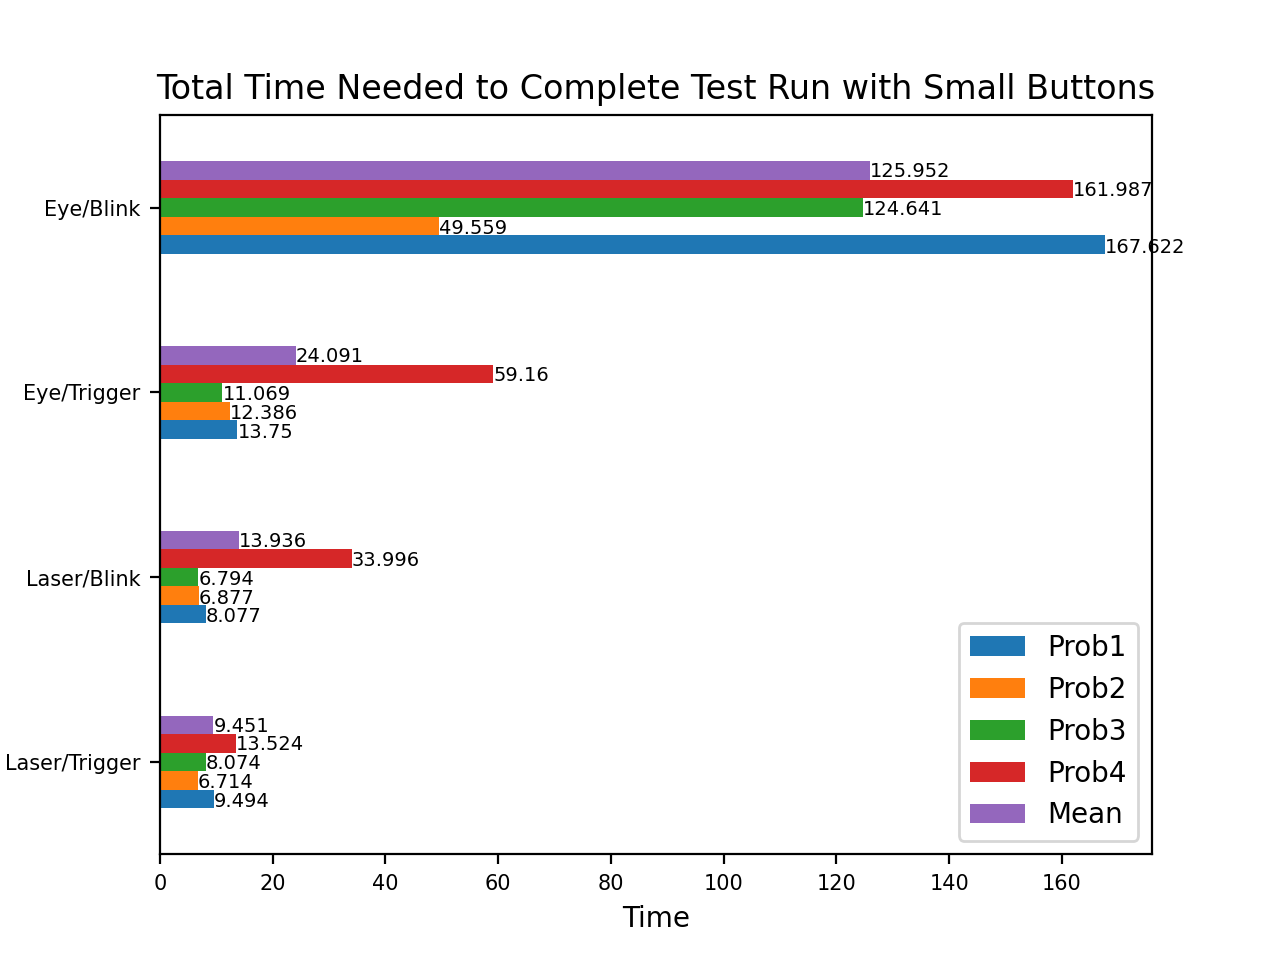
\includegraphics[width=1.0\linewidth]{plot_small}
	\caption[Gesamtdauer eines Versuchdurchlaufs pro Steuerart pro Proband und im Durchschnitt bei kleinen Knöpfen] {Gesamtdauer eines Versuchdurchlaufs pro Steuerart pro Proband und im Durchschnitt bei kleinen Knöpfen}
\end{figure}

\section{Eye-Tracking Heatmaps der Probandenversuche}
\label{appendix:heatmaps}
\begin{figure}[!htbp]
	\centering
	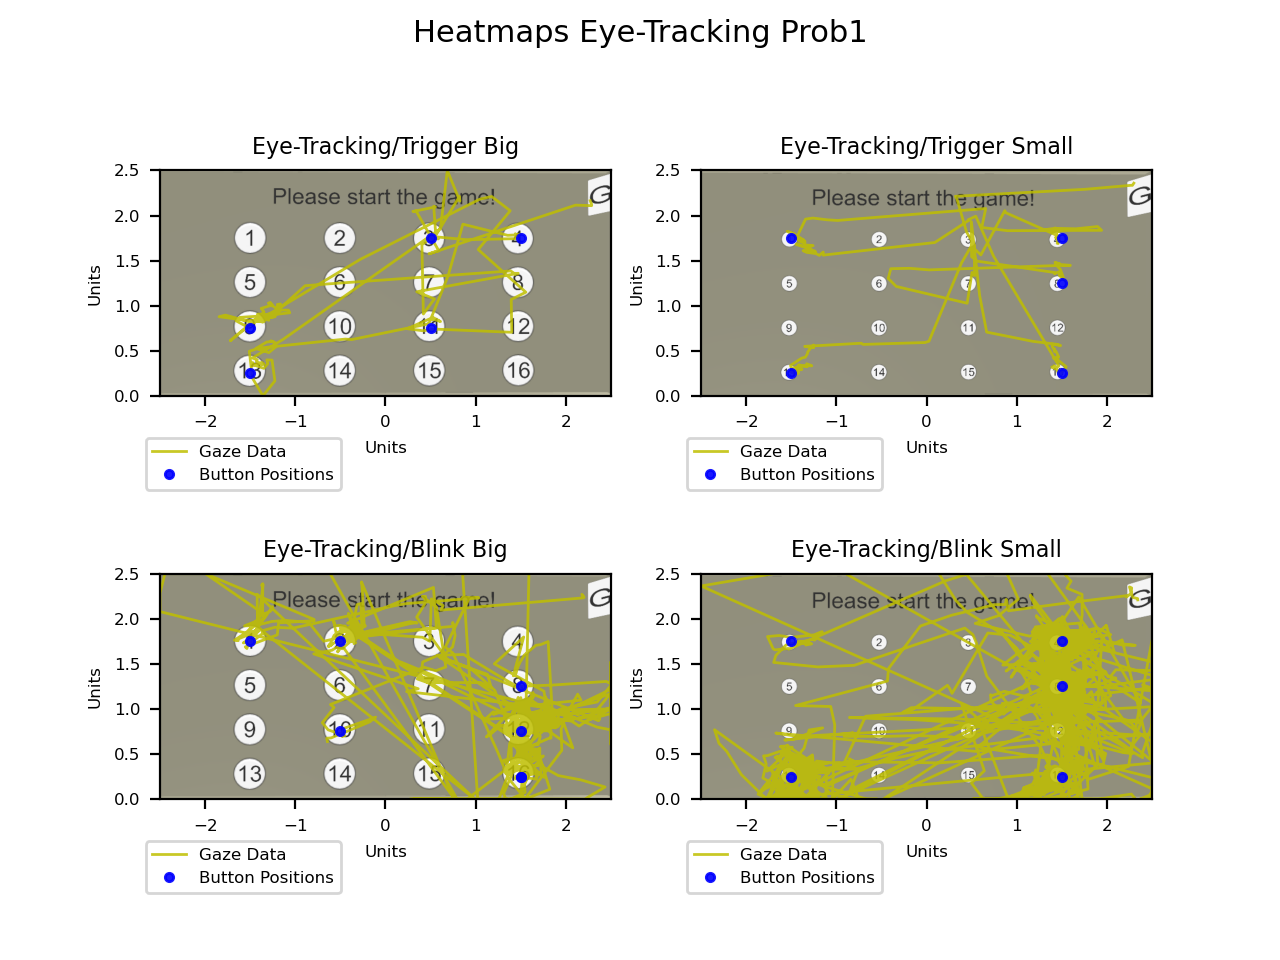
\includegraphics[width=1.0\linewidth]{plot_heatmap_prob1}
	\caption[Visualisierung der Blickdaten und der auszuwählenden Knöpfe] {Visualisierung der Blickdaten und der auszuwählenden Knöpfe}
\end{figure}
\begin{figure}[!htbp]
	\centering
	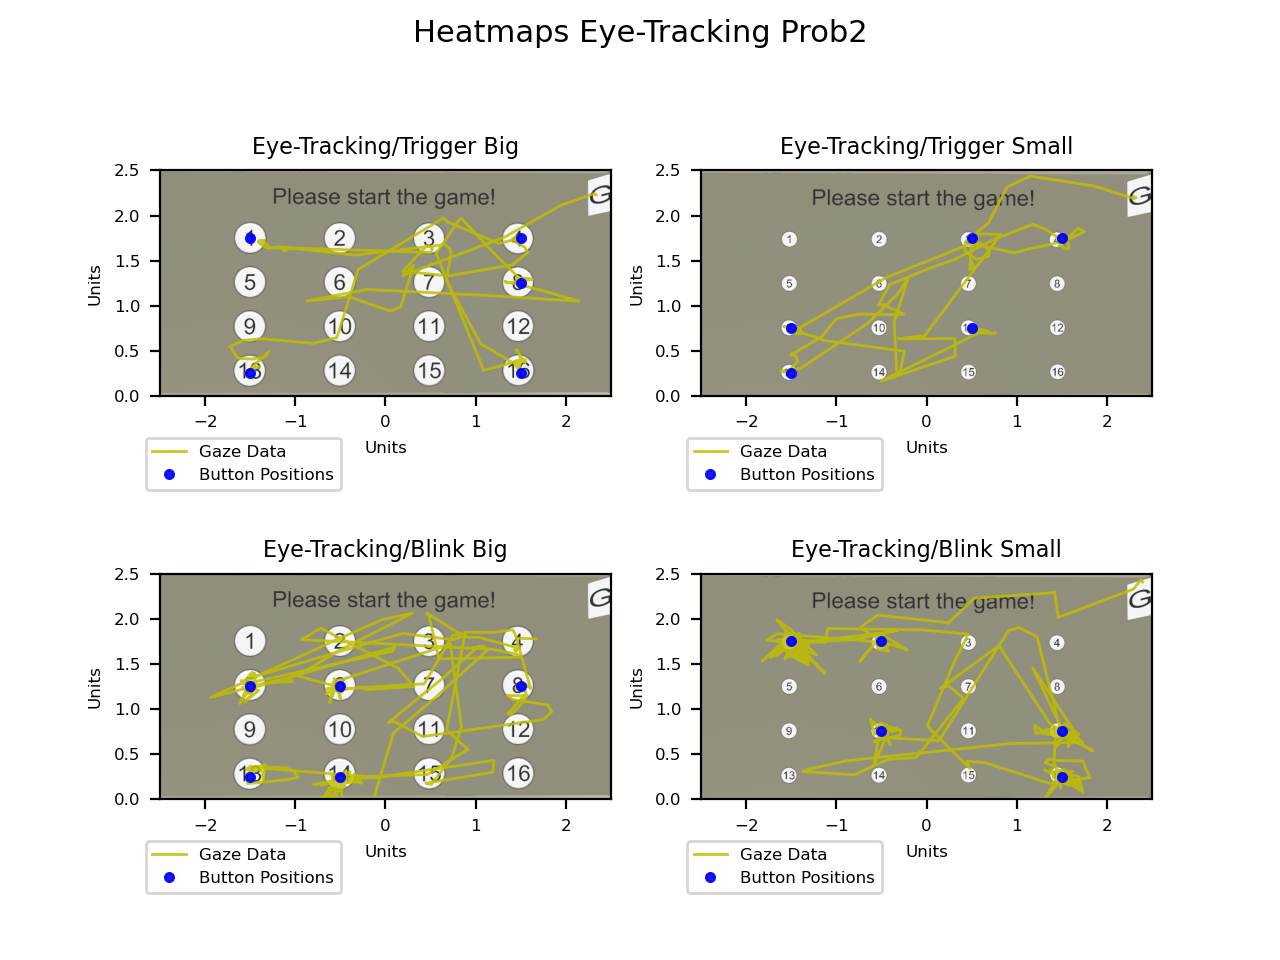
\includegraphics[width=1.0\linewidth]{plot_heatmap_prob2}
	\caption[Visualisierung der Blickdaten und der auszuwählenden Knöpfe] {Visualisierung der Blickdaten und der auszuwählenden Knöpfe}
\end{figure}
\begin{figure}[!htbp]
	\centering
	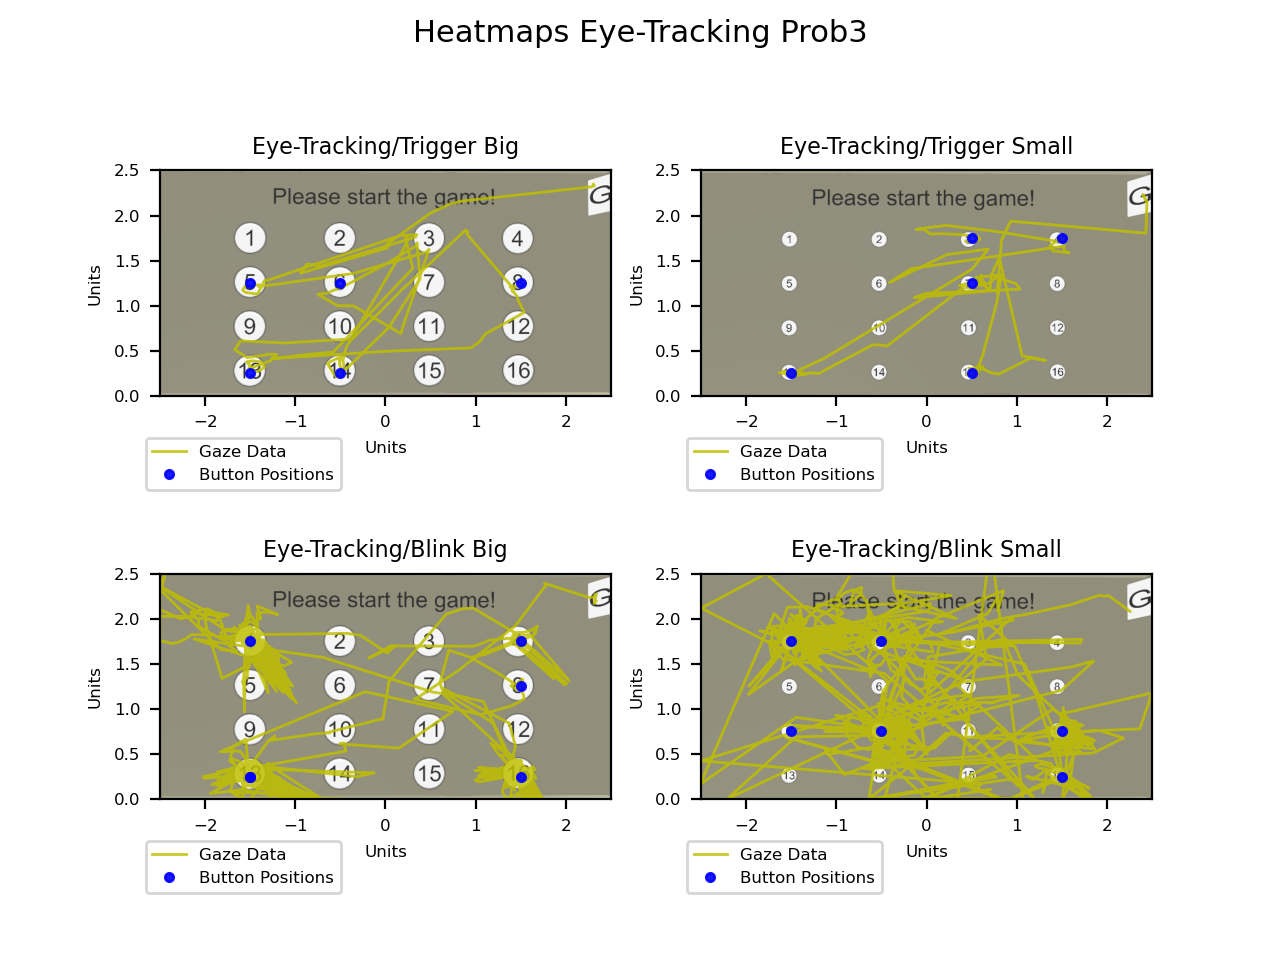
\includegraphics[width=1.0\linewidth]{plot_heatmap_prob3}
	\caption[Visualisierung der Blickdaten und der auszuwählenden Knöpfe] {Visualisierung der Blickdaten und der auszuwählenden Knöpfe}
\end{figure}
\begin{figure}[!htbp]
	\centering
	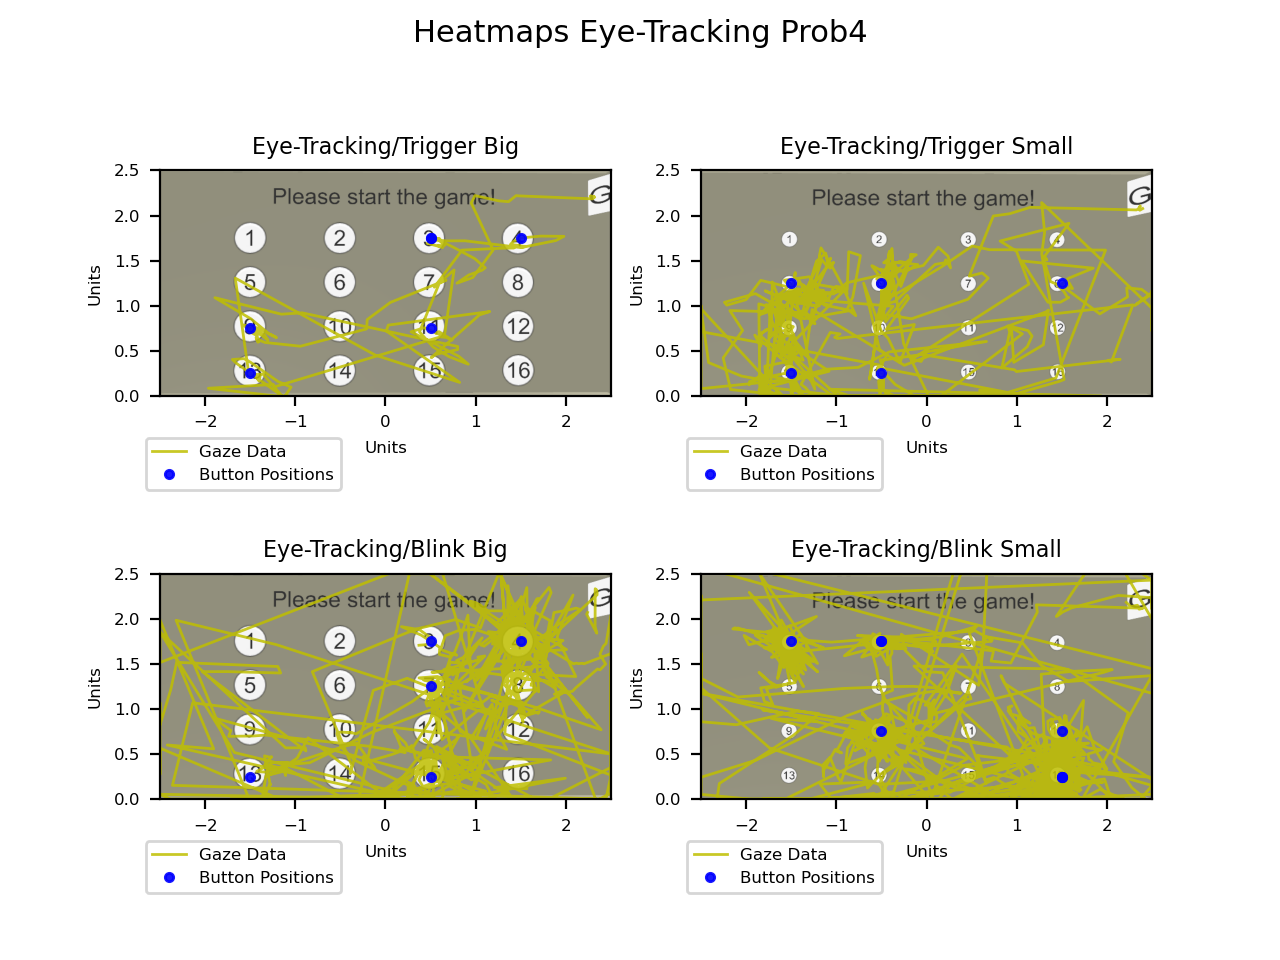
\includegraphics[width=1.0\linewidth]{plot_heatmap_prob4}
	\caption[Visualisierung der Blickdaten und der auszuwählenden Knöpfe] {Visualisierung der Blickdaten und der auszuwählenden Knöpfe}
\end{figure}

\section{Fragebogen}
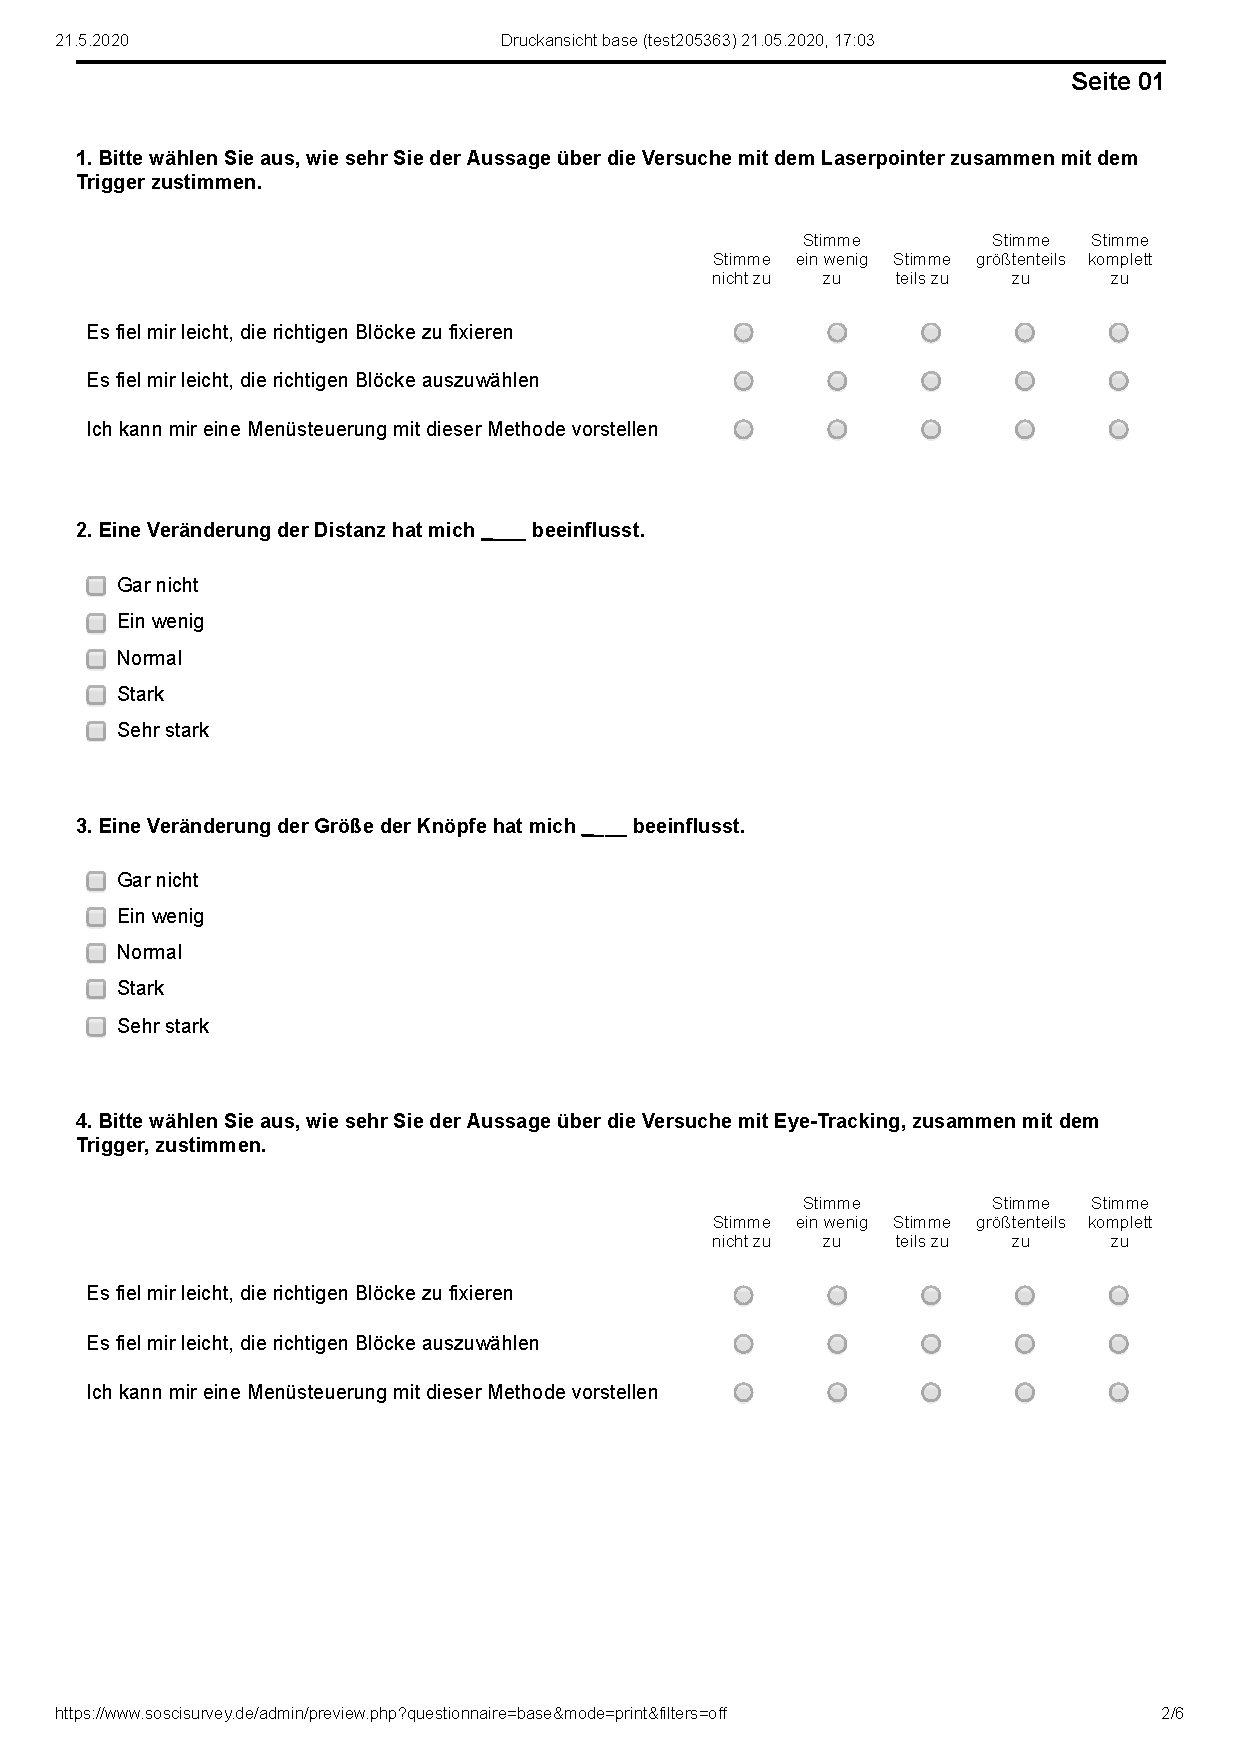
\includepdf[pages=-]{fragebogen.pdf}